\documentclass[preprint]{elsarticle}

\usepackage{amsmath}%
\usepackage{amsfonts}%
\usepackage{amssymb}%
\usepackage{dsfont}
%\usepackage{graphicx}
%\usepackage[latin1]{inputenc} 
%\usepackage[T1]{fontenc} 
%\usepackage{layout}
%\usepackage{setspace}
\usepackage{pgf,tikz}
\usepackage{subcaption}
\captionsetup{compatibility=false}
\usepackage[lined, ruled]{algorithm2e}
\usepackage{enumitem}
%\usepackage[left=2.6cm,right=2.6cm,top=2cm,bottom=3cm]{geometry}
%\usepackage{authblk}


\usetikzlibrary{decorations}
\usetikzlibrary{decorations.pathmorphing}
\usetikzlibrary{decorations.pathreplacing}
\usetikzlibrary{decorations.shapes}
\usetikzlibrary{decorations.text}
\usetikzlibrary{decorations.markings}
\usetikzlibrary{decorations.fractals}
\usetikzlibrary{decorations.footprints}

\usetikzlibrary{arrows}

\newtheorem{theorem}{Theorem}
\newtheorem{definition}{Definition}
\newtheorem{lemma}{Lemma}
\newtheorem{example}{Example}
\newtheorem{corollary}{Corollary}
\newtheorem{problem}{Problem}
\newtheorem{acknowledgement}[theorem]{Acknowledgement}
\newtheorem{axiom}[theorem]{Axiom}
\newtheorem{case}[theorem]{Case}
\newtheorem{claim}[theorem]{Claim}
\newtheorem{conclusion}[theorem]{Conclusion}
\newtheorem{condition}[theorem]{Condition}
\newtheorem{conjecture}[theorem]{Conjecture}

\newtheorem{criterion}[theorem]{Criterion}
\newtheorem{exercise}[theorem]{Exercise}
\newtheorem{notation}[theorem]{Notation}
\newtheorem{proposition}[theorem]{Proposition}
\newtheorem{remark}[theorem]{Remark}
\newtheorem{solution}[theorem]{Solution}
\newtheorem{summary}[theorem]{Summary}
\newenvironment{proof}[1][Proof]{\textbf{#1.} }{\ \rule{0.5em}{0.5em}}

\newcommand{\kctp}{$k$-CTP}
\newcommand{\set}[1]{\left\{ #1 \right\}}
\newcommand{\card}[1]{\left| #1 \right|}
\newcommand{\ith}[1]{#1^{\mbox{\scriptsize{th}}}}
\newcommand{\stpath}{$(s,t)$-path}
\newcommand{\stpaths}{$(s,t)$-paths}
\newcommand{\true}{\mbox{true}}
\newcommand{\false}{\mbox{false}}
\newcommand{\ifend}{\textbf{endif}}
\newcommand{\karp}{=_{\mbox{\scriptsize{K}}}}
\newcommand{\lkarp}{\leq_{\mbox{\scriptsize{K}}}}
\newcommand{\omegamin}{\omega_{\mbox{\scriptsize{min}}}}
\newcommand{\mcale}{\mathcal{E}}
\newcommand{\mcals}{\mathcal{S}}
\newcommand{\mcala}{\mathcal{A}}
\newcommand{\mcalv}{\mathcal{V}}
\newcommand{\mcalg}{\mathcal{G}}
\newcommand{\mcalr}{\mathcal{R}}
\newcommand{\mcald}{\mathcal{D}}
\newcommand{\mcalf}{\mathcal{F}}
\newcommand{\mts}{MS}
\newcommand{\argmin}[1]{\underset{#1}{\operatorname{argmin}}}
\newcommand{\deltavert}{\Delta_{\mbox{\scriptsize{vert}}}}
\newcommand{\Gv}{G^{(v)}}
\newcommand{\caup}{c_A^{\mbox{\scriptsize{up}}}}
\newcommand{\cadown}{c_A^{\mbox{\scriptsize{down}}}}
\newcommand{\cadownbis}{c_{A'}^{\mbox{\scriptsize{down}}}}
\newcommand{\cms}{c_{\mbox{\scriptsize{MS}}}}
\newcommand{\cmsx}[1]{c_{\mbox{\scriptsize{MS}}, #1}}
\newcommand{\cmsr}{c_{\mbox{\scriptsize{MS}}, \mathcal{R}}}
\newcommand{\bintree}{\textsc{bin-tree}}
\newcommand{\ebt}{EBT}
\newcommand{\bfs}{\mbox{BFS}}
\newcommand{\compbin}[1]{\mathcal{C}_{\mbox{\scriptsize{B}}}\left( #1 \right)}
\newcommand{\dmin}{D_{\mbox{\scriptsize{min}}}}
\newcommand{\eleft}[1]{E_{#1, \mbox{\scriptsize{left}}}}
\newcommand{\eright}[1]{E_{#1, \mbox{\scriptsize{right}}}}

\begin{document}

\title{On the competitiveness of memoryless strategies for the Canadian Traveller Problem}
\author[upsud]{Pierre Berg\'e \corref{corrauthor}}
\ead{Pierre.Berge@lri.fr}
\author[cs]{Julien Hemery}
\author[cs]{Arpad Rimmel}
\author[cs]{Joanna Tomasik}
\address[upsud]{LRI, Universit\'e Paris-Sud, Universit\'e Paris-Saclay, 91405 Orsay Cedex, France}
\address[cs]{LRI, CentraleSup\' elec, Universit\'e Paris-Saclay, 91405 Orsay Cedex, France}
\cortext[corrauthor]{Corresponding author}

\begin{abstract}
The $k$-Canadian Traveller Problem, defined and proven PSPACE-complete by Papadimitriou and Yannakakis, is a generalization of the Shortest Path Problem which admits blocked edges. Its objective is to determine the strategy that makes the traveller traverse graph $G$ between two given nodes $s$ and $t$ with the minimal distance, knowing that at most $k$ edges are blocked. The traveller discovers that an edge is blocked when arriving at its endpoint. 
%Westphal showed that the competitive ratio, which is an indicator of the online algorithm quality, of any randomized strategy is not less than $k+1$. 
 
We study the competitiveness of randomized memoryless strategies for the \kctp . In this context, a decision taken by the traveler in node $v$ of $G$ does not depend on its anterior moves. We establish that the competitive ratio of any randomized memoryless strategy cannot be better than $2k + O\left(1\right)$. The primordial consequence of this result is that randomized memoryless strategies are asymptotically as competitive as deterministic strategies which achieve a ratio $2k+1$ at best. In future research, if we aim at designing a strategy with competitive ratio $\alpha k + O\left(1\right)$, $\alpha < 2$, we shall focus on strategies which not only are randomized but also use memory.
\end{abstract}

\maketitle


\section{Introduction}

The \textit{Canadian Traveller Problem} (CTP), a generalization of the \textit{Shortest Path Problem}, was introduced in~\cite{PaYa91}. Given an undirected weighted graph $G=(V,E,\omega)$ and two nodes $s,t \in V$, the objective is to design a strategy to make a traveller walk from $s$ to $t$ through $G$ on the shortest path possible. Its particularity is that some edges of $G$ are potentially blocked. The traveller does not know, however, which edges are blocked. This implies that we solve the CTP with online algorithms, called strategies. He discovers blocked edges, also called blockages, when arriving to its endpoints. The $k$-\textit{Canadian Traveller Problem} (\kctp) is the parameterized variant of CTP, where an upper bound $k$ for the number of blocked edges is given. Both CTP and \kctp ~are PSPACE-complete~\cite{BaSc91,PaYa91}.

\paragraph{State-of-the-art}
Strategies for the \kctp ~are studied through the competitive analysis, which evaluates their quality~\cite{BoEl98}. The competitive ratio of a strategy is the maximum, over every satisfiable instance, of the ratio of the distance traversed by the traveller following the strategy and the \textit{optimal offline cost}, which is the distance he traverses if he knows blocked edges from the beginning. 

There are two classes of strategies: deterministic and randomized. Westphal~\cite{We08} proved that there is no deterministic strategy that achieves a competitive ratio better than $2k+1$. This ratio is reached by \textsc{reposition} and \textsc{comparison} strategies~\cite{We08,XuHuSuZh09}. The \textsc{reposition} strategy consists in traversing the shortest \stpath ~on the current graph. If the traveller discovers that an edge $e^*$ of this path is blocked, he goes back to node $s$ and restarts the process on graph $G$ deprived of the edge $e^*$. 
%Through the competitive analysis point of view, \textsc{reposition} algorithm is an optimal deterministic strategy. 
This algorithm is executed in polynomial time. However, considering specific practical cases such as urban networks, returning to node $s$ every time the traveller is blocked does not seem realistic. This is why Xu {\em et al.\/}~\cite{XuHuSuZh09} introduced the \textsc{greedy} algorithm. For grids, it achieves an $\mathcal{O}\left(1\right)$ ratio, regardless of $k$. However, for any graph, this ratio is $\mathcal{O}\left(2^k\right)$.

We evaluate the competitiveness of the randomized strategies by calculating the maximal ratio of the mean distance traversed by the traveller following the strategy by the optimal offline cost. Westphal~\cite{We08} proved that there is no randomized algorithm that can attain a ratio smaller than $k+1$. However, unlike the deterministic case, no $\left(\alpha k+1\right)$-competitive randomized strategy, $\alpha < 2$, was identified, excepted for very particular cases. Two randomized strategies have been proposed. Demaine {\em et al.\/}~\cite{DeHuLiSa14} designed a strategy with a ratio $\left(1+\frac{\sqrt{2}}{2}\right)k+1$, executed in time of $\mathcal{O}\left(k\mu^2\card{E}^2\right)$ where parameter $\mu$ may be exponential. It is dedicated to graphs that can be transformed into apex trees. 
%It provides a $\left(k+1\right)$-competitive strategy for graphs $G$ which are apex trees with equal-weight \stpaths . 
Bender {\em et al.\/} studied in~\cite{BeWe15} a restriction of \kctp ~for graphs composed of node-disjoint \stpaths ~and proposed a polynomial-time strategy with ratio $\left(k+1\right)$. 

\paragraph{Contributions and paper plan}
We study the competitiveness of memoryless strategies~\cite{Al03,BoEl98}. The choice the traveller makes at node $v$ (to decide where to go next) is independent of his travel before reaching node $v$. 
Given that deterministic memoryless strategies cannot achieve a ratio better than $2k+1$, our goal is to prove that randomized memoryless strategies are not more competitive asymptotically. To do this, we identify a lower bound $c_k = 2k + O\left(1\right)$ of the competitiveness of randomized memoryless strategies for the \kctp.

We remind, in Section~\ref{sec:def}, the definitions of \kctp , memoryless strategies and the competitive ratio.
In Section~\ref{sec:roadatlas}, we present a set $\mathcal{R}$ (called a road atlas) of \textit{road maps}, {\em i.e.} pairs $\left(G,E_*\right)$ with graph $G$ and blocked edges $E_*$, on which we study the competitiveness of memoryless strategies. We associate, to any of these road maps, a binary tree representation which allows to understand the behavior of memoryless strategies on these road maps more comfortably.
We prove in Section~\ref{sec:competitiveness} that randomized memoryless strategies cannot drop below a ratio $c_k = 2k+O\left(1\right)$ on road maps in $\mathcal{R}$. We also clarify expression $O\left(1\right)$ in order to specify the asymptotic behavior of sequence $c_k$.
Eventually, we draw conclusions and highlight the future work in Section~\ref{sec:conclusion}.
%\begin{itemize}
%\item Proof, in Section~\ref{sec:notk+1}, that there is no randomized memoryless strategy which has a ratio $f(k) \leq k+1$ for the \kctp{}.
%\item Establishing, in Section~\ref{sec:compratio}, a bound on the competitive ratio of memoryless strategies. There is no memoryless strategy that solves the \kctp ~with a ratio less than $k\beta + 1$ with $\beta = 3-\sqrt{3} \approx 1.268$. This implies that, if a randomized strategy has a ratio smaller than $k\beta+1$ for any graph, it is not memoryless.
%\end{itemize}
\section{Definitions} \label{sec:def}

We start by introducing the notation. For any graph $G=\left(V,E,\omega\right)$, let $G\backslash E'$ denotes its subgraph $\left(V,E\backslash E',\omega\right)$. 
%If $P$ is a path, we note its cost as $\omega\left(P\right) = \sum_{e \in P} \omega(e)$. 

\subsection{Memoryless Strategies for the \kctp} \label{subsec:msintro}

We remind the definition of CTP. Let $G=\left(V,E,\omega\right)$ be an undirected graph with positive weights. The objective is to make a traveller traverse the graph from a source node $s$ to a target one $t$, with $s,t \in V$. There is a set $E_* \subsetneq E$ of blocked edges. %Without blocked edges, the remaining graph can be still traversed by the traveller: there exists a \stpath ~in graph $G\backslash E_* = \left(V,E\backslash E_*\right)$. 
The traveller does not know a priori which edges are blocked. He discovers a blocked edge only when arriving to one of its endpoints. For example, if $\left(v,w\right)$ is a blockage he will discover it when arriving to $v$ (or $w$). The goal is to design the strategy $A$ with the minimal competitive ratio.
%\begin{figure}[t]
%\centering
%\includegraphics[scale=0.27]{graphics/illustrateCTP2.pdf}
%\caption{Illustration of the \textsc{greedy} strategy on a graph with 2 blocked edges}
%\label{fig:illustrateCTP}
%\end{figure}

We focus on \textit{memoryless strategies} (\mts). Concretely, we suppose that the traveller remembers the blocked edges he has discovered but forgets the nodes which he has already visited. In other words, a decision of an \mts ~is independent of the nodes already visited. In the literature, the term \textit{memoryless} was used in the context of online algorithms (e.g. \textsc{paging problem}~\cite{BoEl98}, \textsc{list update problem}~\cite{Al03}) which take decisions according to the current state, ignoring past events. An \mts ~can be either deterministic or randomized.



\begin{definition}[Memoryless Strategies for the \kctp]
A deterministic strategy $A$ is an \mts ~if and only if (iff) the next node $w$ the traveller visits depends on graph $G$ deprived of blocked edges already discovered $E_*'$ and the current traveller position $v$: $w = A\left(G\backslash E_*',v\right)$. Similarly, a randomized strategy $A$ is an \mts ~iff node $w$ is the realization of a discrete random variable $X = A\left(G\backslash E_*',v\right)$.
\end{definition}

\mts es are easy to be implemented because they do not use past moves to take a decision.
%  For the same reason, they do not need any extra memory either.
For example, the \textsc{greedy} strategy~\cite{XuHuSuZh09} is a deterministic \mts . It consists in choosing at each step the first edge of the shortest path between the current node $v$ and the target~$t$. 
%This strategy, illustrated in Figure~\ref{fig:illustrateCTP}, does not refer to anterior moves. 
In contrast, the \textsc{reposition} strategy~\cite{We08} is not an \mts ~as any decision refers to the past moves of the traveller. The polynomial-time strategies proposed in the literature do not use much memory information in the decision-taking process. Either they are memoryless or they use a weak quantity of memory. For example, \textsc{reposition} (deterministic~\cite{We08} or randomized~\cite{BeWe15}) can be implemented with a  one bit memory given that the only information to retain is whether the traveller tries to reach $t$ or to return to $s$.

The following process allows to identify whether a strategy $A$ is a deterministic \mts . Let us suppose that a traveller $T_1$ executes strategy $A$: he has already visited certain nodes of the graph, he is currently at node $v$ but he has not reached target $t$ yet. Let us imagine a second traveller $T_2$ who is airdropped on node $v$ and starts applying strategy $A$. If the traveller $T_2$ always follows the same path as $T_1$ until reaching $t$, $A$ is a deterministic \mts . If $T_1$ and $T_2$ may follow different paths, then $A$ is not an \mts . Formally, prooving that a strategy is a \mts ~consists in finding the function which transforms the pair $\left(G\backslash E_*,v\right)$ into node $w = A\left(G\backslash E_*',v\right)$.

\subsection{Competitive ratio} \label{subsec:compratio}

Let $\left(G,E_*\right)$ be a \textit{road map}, {\em i.e.} a pair with graph $G=\left(V,E,\omega\right)$ and blocked edges $E_* \subsetneq E$, such that there is an \stpath ~in graph $G\backslash E_*$ (nodes $s$ and $t$ remain in the same connected component when all blocked edges are discovered). We note $\omega_A\left(G,E_*\right)$ the distance traversed by the traveller reaching $t$ with strategy $A$ on graph $G$ with blocked edges $E_*$ and $\omegamin\left(G,E_*\right)$ the cost of the shortest \stpath ~in graph $G\backslash E_*$.

The ratio $\omega_A\left(G,E_*\right)/\omegamin\left(G,E_*\right)$ is abbreviated as $c_A\left(G,E_*\right)$. A strategy $A$ is $c_A$-competitive~\cite{BoEl98,XuHuSuZh09} iff for any $\left(G,E_*\right), \omega_A\left(G,E_*\right) \leq c_A \omegamin\left(G,E_*\right)$. Otherwise stated, for any $\left(G,E_*\right)$, $c_A\left(G,E_*\right) \leq c_A$. If strategy $A$ is randomized, $\omega_A\left(G,E_*\right)$ is replaced by $\mathbb{E}\left(\omega_A\left(G,E_*\right)\right)$ which is the expected distance traversed by the traveller to reach $t$ with strategy $A$. The competitive ratio can also be evaluated on a family $\mathcal{R}$ of road maps, put formally,

\begin{equation}
c_{A,\mathcal{R}} = \max\limits_{\left(G,E_*\right) \in \mathcal{R}} c_A\left(G,E_*\right)
\end{equation}

% See command \cms
This ``local'' competitive ratio fulfils $c_{A,\mathcal{R}} \le c_A$. The definition of the competitive ratio can also be extended to families of strategies. We note $\cms$ the competitive ratio of \mts es, which is the minimum over competitive ratios of any \mts es: $\cms = \min\limits_{A ~\mbox{\scriptsize{\mts}}} c_A$. In the remainder, we identify a set of road maps $\mathcal{R}$ such that the competitive ratio of \mts es on it is $2k+O\left(1\right)$.

\section{Road atlas used to study randomized \mts es} \label{sec:roadatlas}

We specify a \textit{road atlas} $\mathcal{R}$, {\em i.e.} a set of road maps, which will be used to evaluate the competitiveness of randomized \mts es. We introduce a family of graphs $G_i$ such that graphs composing this road atlas are subgraphs of $G_i$. 

\subsection{Graphs composing the road atlas $\mcalr$} \label{subsec:Gi}

We define recursively a sequence of graphs $G_i$ for $i \geq 1$ with weights from $\set{1,\varepsilon}$, $0 < \varepsilon \ll 1$. Graphs $G_1$ and $G_{i+1}$ are represented in Figures~\ref{subfig:G_1} and~\ref{subfig:G_i}, respectively. Graphs $G_2$ and $G_3$ are shown in Figure~\ref{subfig:G_2} and~\ref{subfig:G_3}. Edges with weight 1 are thicker than edges with weight $\varepsilon$. On any graph $G_i$, axis $\deltavert$ is the vertical axis of symmetry (see Figures~\ref{subfig:G_2} and~\ref{subfig:G_3}).

%\begin{figure}[b]
%\centering
%\begin{subfigure}[b]{0.49\columnwidth}
%\centering
%\scalebox{.32}{\input{graphics/deadend_1}}
%\caption{Graph $G_2$ deprived of one edge makes appear a dead end (blue dashed box)}
%\label{subfig:deadend_1}
%\end{subfigure}
%\begin{subfigure}[b]{0.49\columnwidth}
%\centering
%\scalebox{.52}{\input{graphics/deadend_2}}
%\caption{The graph obtained after deleting all nodes\slash edges forming a dead end}
%\label{subfig:deadend_2}
%\end{subfigure}
%\caption{An illustration of dead ends on graph $G_2$.}
%\end{figure}

We focus on the behavior of a traveller traversing road maps $\left(G_k,E_*\right)$ composed of graph $G_k$ and at most $k$ blocked edges $E_*$ at the right of axis $\deltavert$ in graph $G_k$. Indeed, blocking edges left to $\deltavert$ affects negligibly the total distance traversed by a traveller. Let us suppose that the traveller traverses graph $G_k$ and has already discovered some blocked edges $E' \subseteq E_*$. He tries now to reach $t$ on graph $G_k\backslash E'$, ignoring that the undiscovered blocked edges are $E_*' = E_* \backslash E'$.
We note $\mcalg$ the set of all these subgraphs. Formally, $\mcalg = \bigcup_{k=1}^{+\infty} \mcalg_k ~\mbox{with}~
\mcalg_k = \set{G_k\backslash E' : \card{E'} \leq k}$. Road maps $\left(G,E_*\right)$ in $\mcalr$ are composed of graphs in $\mcalg$. For any graph $G \in \mcalg$, we partition its edges, noted $E_G$, in two sets $\eleft{G}$ (left to axis $\deltavert$) and $\eright{G}$ (right to axis $\deltavert$).

\begin{figure}[h]
\centering
\begin{subfigure}[b]{0.49\columnwidth}
\centering
\scalebox{.52}{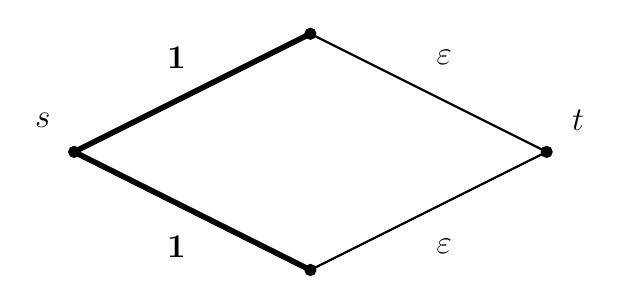
\begin{tikzpicture}[line cap=round,line join=round,>=triangle 45,x=1cm,y=1cm]
%\clip(-6.982493065694897,-13.63448020945784) rectangle (22.448157265896512,6.751180862658525);
\draw [line width=2pt] (0,0)-- (3,1.5);
\draw [line width=0.8pt] (3,1.5)-- (6,0);
\draw [line width=2pt] (0,0)-- (3,-1.5);
\draw [line width=0.8pt] (3,-1.5)-- (6,0);
\begin{scriptsize}\draw [fill=black] (6,0) circle (2pt);
\draw[color=black] (6.4,0.4) node {\large $t$};
\draw [fill=black] (0,0) circle (2pt);
\draw[color=black] (-0.4,0.4) node {\large $s$};
\draw [fill=black] (3,1.5) circle (2pt);
\draw [fill=black] (3,-1.5) circle (2pt);
\draw[color=black] (1.3,1.2) node {\large \bf{1}};
\draw[color=black] (4.7,1.2) node {\large $\varepsilon$};
\draw[color=black] (1.3,-1.2) node {\large \bf{1}};
\draw[color=black] (4.7,-1.2) node {\large $\varepsilon$};
\end{scriptsize}
\end{tikzpicture} }
\caption{Graph $G_1$}
\label{subfig:G_1}
\end{subfigure}
\begin{subfigure}[b]{0.49\columnwidth}
\centering
\scalebox{.52}{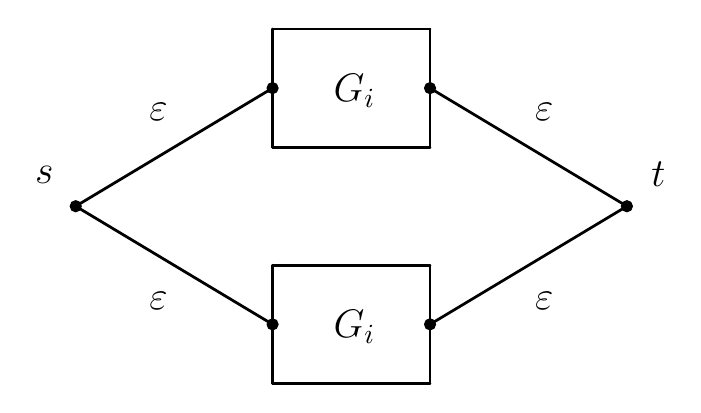
\begin{tikzpicture}[line cap=round,line join=round,>=triangle 45,x=1cm,y=1cm]
\draw [line width=1pt] (0,0)-- (2.5,1.5);
\draw [line width=1pt] (4.5,1.5)-- (7,0);
\draw [line width=1pt] (0,0)-- (2.5,-1.5);
\draw [line width=1pt] (4.5,-1.5)-- (7,0);
\draw [line width=1pt] (2.5,2.25)-- (2.5,0.75);
\draw [line width=1pt] (2.5,0.75)-- (4.5,0.75);
\draw [line width=1pt] (4.5,0.75)-- (4.5,2.25);
\draw [line width=1pt] (4.5,2.25)-- (2.5,2.25);
\draw [line width=1pt] (2.5,-0.75)-- (2.5,-2.25);
\draw [line width=1pt] (2.5,-2.25)-- (4.5,-2.25);
\draw [line width=1pt] (4.5,-2.25)-- (4.5,-0.75);
\draw [line width=1pt] (4.5,-0.75)-- (2.5,-0.75);

\draw (3.15,1.8) node[anchor=north west] {\Large $G_i$};
\draw (3.15,-1.2) node[anchor=north west] {\Large $G_i$};

\begin{scriptsize}

\draw [fill=black] (0,0) circle (2pt);
\draw[color=black] (-0.4,0.4) node {\Large $s$};
\draw [fill=black] (7,0) circle (2pt);
\draw[color=black] (7.4,0.4) node {\Large $t$};
\draw [fill=black] (2.5,1.5) circle (2pt);
\draw [fill=black] (4.5,1.5) circle (2pt);
\draw [fill=black] (2.5,-1.5) circle (2pt);
\draw [fill=black] (4.5,-1.5) circle (2pt);
\draw[color=black] (1.05,1.2) node {\Large $\varepsilon$};
\draw[color=black] (5.95,1.2) node {\Large $\varepsilon$};
\draw[color=black] (1.05,-1.2) node {\Large $\varepsilon$};
\draw[color=black] (5.95,-1.2) node {\Large $\varepsilon$};

\end{scriptsize}
\end{tikzpicture}}
\caption{Graph $G_{i+1}$}
\label{subfig:G_i}
\end{subfigure}
\begin{subfigure}[b]{0.49\columnwidth}
\centering
\scalebox{.45}{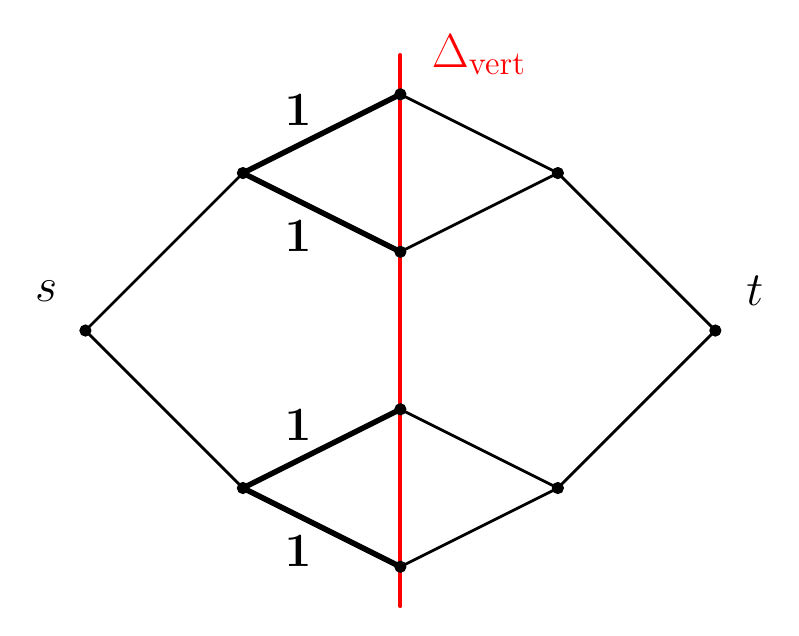
\begin{tikzpicture}[line cap=round,line join=round,>=triangle 45,x=1cm,y=1cm]
%\clip(-7.415949195666677,-4.979207164201812) rectangle (6.110862528225963,7.380468149885891);
\draw [line width=1pt] (0,0)-- (2,2);
\draw [line width=2pt] (2,2)-- (4,3);
\draw [line width=2pt] (2,2)-- (4,1);
\draw [line width=1pt] (4,3)-- (6,2);
\draw [line width=1pt] (4,1)-- (6,2);
\draw [line width=1pt] (6,2)-- (8,0);
\draw [line width=1pt] (0,0)-- (2,-2);
\draw [line width=2pt] (2,-2)-- (4,-3);
\draw [line width=2pt] (2,-2)-- (4,-1);
\draw [line width=1pt] (4,-3)-- (6,-2);
\draw [line width=1pt] (4,-1)-- (6,-2);
\draw [line width=1pt] (6,-2)-- (8,0);
\begin{scriptsize}
\draw [line width = 1.4pt,color=red] (4,3.5)--(4,-3.5);
\draw[color=red] (5,3.5) node {\LARGE $\Delta_{\mbox{\large vert}}$};
\draw [fill=black] (2, 2) circle (2pt);
\draw [fill=black] (4, 3) circle (2pt);
\draw [fill=black] (6, 2) circle (2pt);
\draw [fill=black] (4, 1) circle (2pt);
\draw [fill=black] (0, 0) circle (2pt);
\draw [fill=black] (8, 0) circle (2pt);
\draw [fill=black] (2, -2) circle (2pt);
\draw [fill=black] (4, -3) circle (2pt);
\draw [fill=black] (6, -2) circle (2pt);
\draw [fill=black] (4, -1) circle (2pt);
\draw[color=black] (-0.5, 0.5) node {\LARGE $s$};
\draw[color=black] (2.7, 2.8) node {\LARGE \textbf{1}};
\draw[color=black] (2.7, 1.2) node {\LARGE \textbf{1}};
\draw[color=black] (2.7, -1.2) node {\LARGE \textbf{1}};
\draw[color=black] (2.7, -2.8) node {\LARGE \textbf{1}};
\draw[color=black] (8.5, 0.5) node {\LARGE $t$};
\end{scriptsize}
\end{tikzpicture}
}
\caption{Graph $G_2$ and axis $\deltavert$}
\label{subfig:G_2}
\end{subfigure}
\begin{subfigure}[b]{0.49\columnwidth}
\centering
\scalebox{0.45}{%\begin{tikzpicture}[line cap=round,line join=round,>=triangle 45,x=1cm,y=1cm]
%%\clip(-7.415949195666677,-5.90693097712365) rectangle (20.34094875546258,7.380468149885891);
%\draw [line width=1pt] (-4.0,2.5)-- (-2.5,4);
%\draw [line width=1pt] (0.5,4)-- (2.0,2.5);
%\draw [line width=1pt] (0.5,1)-- (2.0,2.5);
%\draw [line width=1pt] (-4.0,2.5)-- (-2.5,1);
%\draw [line width=1pt] (-2.5,4)-- (-1.4,4.6);
%\draw [line width=2pt] (-1.4,4.6)-- (-1,5);
%\draw [line width=1pt] (-1,5)-- (-0.6,4.6);
%\draw [line width=1pt] (-0.6,4.6)-- (-1,4.2);
%\draw [line width=2pt] (-1.4,4.6)-- (-1,4.2);
%\draw [line width=1pt] (-0.6,4.6)-- (0.5,4);
%\draw [line width=1pt] (-2.5,4)-- (-1.4,3.4);
%\draw [line width=2pt] (-1.4,3.4)-- (-1,3.8);
%\draw [line width=1pt] (-1,3.8)-- (-0.6,3.4);
%\draw [line width=2pt] (-1.4,3.4)-- (-1,3);
%\draw [line width=1pt] (-1,3)-- (-0.6,3.4);
%\draw [line width=1pt] (-0.6,3.4)-- (0.5,4);
%\draw [line width=1pt] (-2.5,1)-- (-1.4,1.6);
%\draw [line width=2pt] (-1.4,1.6)-- (-1,2);
%\draw [line width=2pt] (-1.4,1.6)-- (-1,1.2);
%\draw [line width=1pt] (-1,1.2)-- (-0.6,1.6);
%\draw [line width=1pt] (-1,2)-- (-0.6,1.6);
%\draw [line width=1pt] (-0.6,1.6)-- (0.5,1);
%\draw [line width=1pt] (-2.5,1)-- (-1.4,0.4);
%\draw [line width=2pt] (-1.4,0.4)-- (-1,0.8);
%\draw [line width=1pt] (-1,0.8)-- (-0.6,0.4);
%\draw [line width=2pt] (-1.4,0.4)-- (-1,0);
%\draw [line width=1pt] (-1,0)-- (-0.6,0.4);
%\draw [line width=1pt] (-0.6,0.4)-- (0.5,1);
%\begin{scriptsize}
%\draw [line width = 1.4pt,color=red] (-1,-0.6)--(-1,5.6);
%\draw[color=red] (-0.5,5.8) node {$\deltavert$};
%\draw [fill=black] (0.5,4) circle (2pt);
%\draw [fill=black] (-2.5,4) circle (2pt);
%\draw [fill=black] (-1.4,4.6) circle (1.5pt);
%\draw [fill=black] (-1.4,3.4) circle (1.5pt);
%\draw [fill=black] (-4.0,2.5) circle (1.5pt);
%\draw[color=black] (-4.3,2.7) node {$s$};
%\draw [fill=black] (2.0,2.5) circle (1.5pt);
%\draw[color=black] (2.4,2.7) node {$t$};
%\draw [fill=black] (-2.5,1) circle (1.5pt);
%\draw [fill=black] (-1.4,1.6) circle (1.5pt);
%\draw [fill=black] (0.5,1) circle (1.5pt);
%\draw [fill=black] (-0.6,0.4) circle (1.5pt);
%\draw [fill=black] (-0.6,1.6) circle (1.5pt);
%\draw [fill=black] (-1.4,0.4) circle (1.5pt);
%\draw [fill=black] (-1,2) circle (1.5pt);
%\draw [fill=black] (-1,1.2) circle (1.5pt);
%\draw [fill=black] (-1,0.8) circle (1.5pt);
%\draw [fill=black] (-1,0) circle (1.5pt);
%\draw [fill=black] (-0.6,4.6) circle (1.5pt);
%\draw [fill=black] (-1,5) circle (1.5pt);
%\draw [fill=black] (-1,4.2) circle (1.5pt);
%\draw [fill=black] (-1,3.8) circle (1.5pt);
%\draw [fill=black] (-1,3) circle (1.5pt);
%\draw [fill=black] (-0.6,3.4) circle (1.5pt);
%\draw[color=black] (-1.3,5) node {1};
%\draw[color=black] (-1.3,4.2) node {1};
%\draw[color=black] (-1.3,3.8) node {1};
%\draw[color=black] (-1.3,3) node {1};
%\draw[color=black] (-1.3,2) node {1};
%\draw[color=black] (-1.3,1.2) node {1};
%\draw[color=black] (-1.3,0.8) node {1};
%\draw[color=black] (-1.3,0) node {1};
%\end{scriptsize}
%\end{tikzpicture}


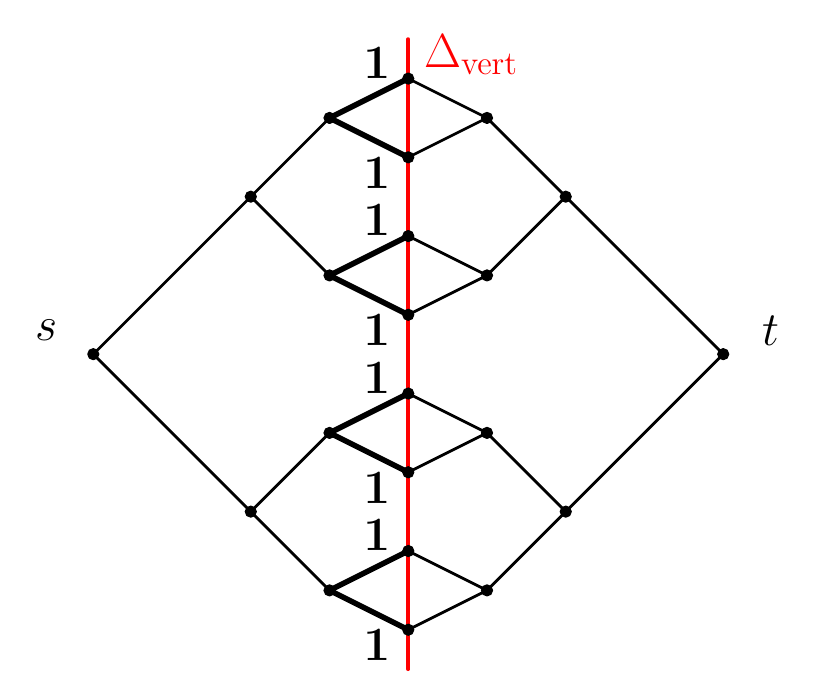
\begin{tikzpicture}[line cap=round,line join=round,>=triangle 45,x=1cm,y=1cm]
%\clip(-7.415949195666677,-4.979207164201812) rectangle (6.110862528225963,7.380468149885891);
\draw [line width=1pt] (-1,0)-- (1,2);
\draw [line width=1pt] (1,2)-- (2,3);
\draw [line width=2pt] (2,3)-- (3,3.5);
\draw [line width=2pt] (2,3)-- (3,2.5);
\draw [line width=1pt] (3,3.5)-- (4,3);
\draw [line width=1pt] (3,2.5)-- (4,3);
\draw [line width=1pt] (4,3)-- (5,2);
\draw [line width=1pt] (1,2)-- (2,1);
\draw [line width=2pt] (2,1)-- (3,0.5);
\draw [line width=2pt] (2,1)-- (3,1.5);
\draw [line width=1pt] (3,0.5)-- (4,1);
\draw [line width=1pt] (3,1.5)-- (4,1);
\draw [line width=1pt] (4,1)-- (5,2);
\draw [line width=1pt] (5,2)-- (7,0);
\draw [line width=1pt] (-1,0)-- (1,-2);
\draw [line width=1pt] (1,-2)-- (2,-3);
\draw [line width=2pt] (2,-3)-- (3,-3.5);
\draw [line width=2pt] (2,-3)-- (3,-2.5);
\draw [line width=1pt] (3,-3.5)-- (4,-3);
\draw [line width=1pt] (3,-2.5)-- (4,-3);
\draw [line width=1pt] (4,-3)-- (5,-2);
\draw [line width=1pt] (1,-2)-- (2,-1);
\draw [line width=2pt] (2,-1)-- (3,-0.5);
\draw [line width=2pt] (2,-1)-- (3,-1.5);
\draw [line width=1pt] (3,-0.5)-- (4,-1);
\draw [line width=1pt] (3,-1.5)-- (4,-1);
\draw [line width=1pt] (4,-1)-- (5,-2);
\draw [line width=1pt] (5,-2)-- (7,0);
\begin{scriptsize}
\draw [line width = 1.4pt,color=red] (3,4)--(3,-4);
\draw[color=red] (3.8,3.8) node {\LARGE $\Delta_{\mbox{\large vert}}$};
\draw [fill=black] (-1, 0) circle (2pt);
\draw [fill=black] (1, 2) circle (2pt);
\draw [fill=black] (2, 3) circle (2pt);
\draw [fill=black] (3, 3.5) circle (2pt);
\draw [fill=black] (3, 2.5) circle (2pt);
\draw [fill=black] (4, 3) circle (2pt);
\draw [fill=black] (2, 1) circle (2pt);
\draw [fill=black] (3, 1.5) circle (2pt);
\draw [fill=black] (3, 0.5) circle (2pt);
\draw [fill=black] (4, 1) circle (2pt);
\draw [fill=black] (5, 2) circle (2pt);
\draw [fill=black] (1, -2) circle (2pt);
\draw [fill=black] (2, -3) circle (2pt);
\draw [fill=black] (3, -3.5) circle (2pt);
\draw [fill=black] (3, -2.5) circle (2pt);
\draw [fill=black] (4, -3) circle (2pt);
\draw [fill=black] (2, -1) circle (2pt);
\draw [fill=black] (3, -1.5) circle (2pt);
\draw [fill=black] (3, -0.5) circle (2pt);
\draw [fill=black] (4, -1) circle (2pt);
\draw [fill=black] (5, -2) circle (2pt);
\draw [fill=black] (7, 0) circle (2pt);
\draw[color=black] (-1.6, 0.3) node {\LARGE $s$};
\draw[color=black] (2.6, 3.7) node {\LARGE \textbf{1}};
\draw[color=black] (2.6, 2.3) node {\LARGE \textbf{1}};
\draw[color=black] (2.6, 1.7) node {\LARGE \textbf{1}};
\draw[color=black] (2.6, 0.3) node {\LARGE \textbf{1}};
\draw[color=black] (2.6, -0.3) node {\LARGE \textbf{1}};
\draw[color=black] (2.6, -1.7) node {\LARGE \textbf{1}};
\draw[color=black] (2.6, -2.3) node {\LARGE \textbf{1}};
\draw[color=black] (2.6, -3.7) node {\LARGE \textbf{1}};
\draw[color=black] (7.6, 0.3) node {\LARGE $t$};
\end{scriptsize}
\end{tikzpicture}}
\caption{Graph $G_3$ and axis $\deltavert$}
\label{subfig:G_3}
\end{subfigure}
\caption{Recursive construction of graphs $G_i$. Weights $\varepsilon$ are not indicated in Figures~\ref{subfig:G_2} and~\ref{subfig:G_3} to keep them readable.}
\label{fig:G_i}
\end{figure}

%When the traveller discovers blocked edges in a graph $G \in \mcalg_k$, parts of the graph become \textit{dead ends}. If a traveller visits a dead end, the only chance for him to reach $t$ is to leave it anyway. Dead ends only provide to the traveller additional costs which make the competitive ratio increase. Therefore, the most competitive strategies (memoryless or not) do not visit dead ends. As soon as a dead end appear when the traveller discovers a blockage, we delete it from the graph. Graph $G\backslash E'$ becomes graph $G$ deprived of both edges $E'$ and dead ends. 
%
%We study the competitiveness of \mts es on the road atlas $\mathcal{R}$ composed of road maps with sub-graphs $G_k \backslash E' \in \mcalg_k$ where $\mcalg_k = \set{G_k\backslash E' : \card{E'} \leq k}$ and blocked edges $E_*'$ which fulfil $\card{E'} + \card{E_*'} = k$. Formally,
%\[
%\mathcal{R} = \bigcup\limits_{k=1}^{+\infty} \mathcal{R}_k ~\mbox{with}~ \mathcal{R}_k = \set{\left(G_k\backslash E',E_*'\right): G_k\backslash E' \in \mcalg_k, E' \cap E_*' = \emptyset, \card{E'} + \card{E_*'} = k}
%\]

\subsection{Equivalent binary trees} \label{subsec:ebt}

For any graph $G$ of $\mcalg$, we define an equivalent binary tree (\ebt ) noted $T_G$ which represents all \textit{separations} (notion defined below) from $t$ in graph $G$. We note $T_\varnothing$ the empty tree. Any nonempty tree is a triplet $(v, T_a, T_b)$ with a root $v \in V$ and two subtrees $T_a$ and $T_b$.

\begin{figure}[h]
\centering
\begin{subfigure}[b]{0.33\columnwidth}
\centering
\scalebox{.42}{\input{graphics/ebt_1}}
\caption{Graph $G \in \mcalg_3$}
\label{subfig:ebt_1}
\end{subfigure}
~
\begin{subfigure}[b]{0.33\columnwidth}
\centering
\scalebox{.42}{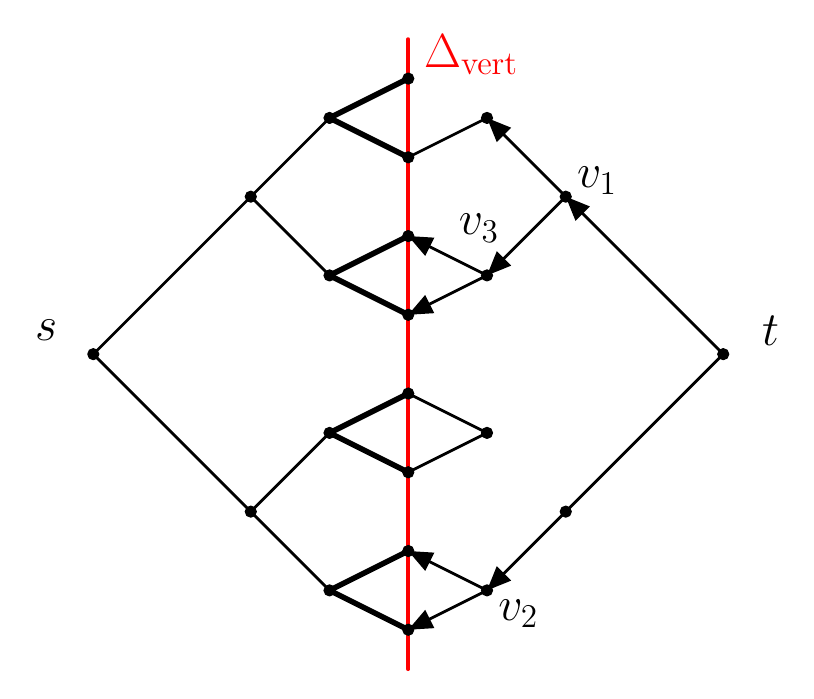
\begin{tikzpicture}[line cap=round,line join=round,>=triangle 45,x=1cm,y=1cm]
%\clip(-7.415949195666677,-4.979207164201812) rectangle (6.110862528225963,7.380468149885891);
\draw [line width=1pt] (-1,0)-- (1,2);
\draw [line width=1pt] (1,2)-- (2,3);
\draw [line width=2pt] (2,3)-- (3,3.5);
\draw [line width=2pt] (2,3)-- (3,2.5);
%\draw [line width=1pt] (3,3.5)-- (4,3);
\draw [line width=1pt,] (3,2.5)-- (4,3);
\draw [line width=1pt,<-] (4,3)-- (5,2);
\draw [line width=1pt] (1,2)-- (2,1);
\draw [line width=2pt] (2,1)-- (3,0.5);
\draw [line width=2pt] (2,1)-- (3,1.5);
\draw [line width=1pt,<-] (3,0.5)-- (4,1);
\draw [line width=1pt,<-] (3,1.5)-- (4,1);
\draw [line width=1pt,<-] (4,1)-- (5,2);
\draw [line width=1pt,<-] (5,2)-- (7,0);
\draw [line width=1pt] (-1,0)-- (1,-2);
\draw [line width=1pt] (1,-2)-- (2,-3);
\draw [line width=2pt] (2,-3)-- (3,-3.5);
\draw [line width=2pt] (2,-3)-- (3,-2.5);
\draw [line width=1pt,<-] (3,-3.5)-- (4,-3);
\draw [line width=1pt,<-] (3,-2.5)-- (4,-3);
\draw [line width=1pt,<-] (4,-3)-- (5,-2);
\draw [line width=1pt] (1,-2)-- (2,-1);
\draw [line width=2pt] (2,-1)-- (3,-0.5);
\draw [line width=2pt] (2,-1)-- (3,-1.5);
\draw [line width=1pt] (3,-0.5)-- (4,-1);
\draw [line width=1pt] (3,-1.5)-- (4,-1);
%\draw [line width=1pt] (4,-1)-- (5,-2);
\draw [line width=1pt] (5,-2)-- (7,0);
\begin{scriptsize}
\draw [line width = 1.4pt,color=red] (3,4)--(3,-4);
\draw[color=red] (3.8,3.8) node {\LARGE $\Delta_{\mbox{\large vert}}$};
\draw [fill=black] (-1, 0) circle (2pt);
\draw [fill=black] (1, 2) circle (2pt);
\draw [fill=black] (2, 3) circle (2pt);
\draw [fill=black] (3, 3.5) circle (2pt);
\draw [fill=black] (3, 2.5) circle (2pt);
\draw [fill=black] (4, 3) circle (2pt);
\draw [fill=black] (2, 1) circle (2pt);
\draw [fill=black] (3, 1.5) circle (2pt);
\draw [fill=black] (3, 0.5) circle (2pt);
\draw [fill=black] (4, 1) circle (2pt);
\draw[color=black] (3.9, 1.6) node {\LARGE $v_3$};
\draw [fill=black] (5, 2) circle (2pt);
\draw[color=black] (5.4, 2.2) node {\LARGE $v_1$};
\draw [fill=black] (1, -2) circle (2pt);
\draw [fill=black] (2, -3) circle (2pt);
\draw [fill=black] (3, -3.5) circle (2pt);
\draw [fill=black] (3, -2.5) circle (2pt);
\draw [fill=black] (4, -3) circle (2pt);
\draw[color=black] (4.4, -3.3) node {\LARGE $v_2$};
\draw [fill=black] (2, -1) circle (2pt);
\draw [fill=black] (3, -1.5) circle (2pt);
\draw [fill=black] (3, -0.5) circle (2pt);
\draw [fill=black] (4, -1) circle (2pt);
\draw [fill=black] (5, -2) circle (2pt);
\draw [fill=black] (7, 0) circle (2pt);
\draw[color=black] (-1.6, 0.3) node {\LARGE $s$};
\draw[color=black] (7.6, 0.3) node {\LARGE $t$};
\end{scriptsize}
\end{tikzpicture}}
\caption{Separations in $G$}
\label{subfig:ebt_2}
\end{subfigure}
~
\begin{subfigure}[b]{0.28\columnwidth}
\centering
\scalebox{.58}{\input{graphics/ebt_3}}
\caption{The EBT $T_G$}
\label{subfig:ebt_3}
\end{subfigure}
\caption{An example of graph $G \in \mcalg_3$ and its EBT $T_G$.}
\label{fig:ebt}
\end{figure}

The EBT is obtained thanks to a breadth-first search (BFS) from $t$ in direction of nodes on axis $\deltavert$. Node $t$ is the root of the EBT. Graphically, each node from which there is a \textit{separation}, {\em i.e.} there are two possible directions for the next move of the BFS, provides two extra branches in the tree (see nodes $t$, $v_1$, $v_2$ and $v_3$ in Figure~\ref{subfig:ebt_2}). Figures~\ref{subfig:ebt_1},~\ref{subfig:ebt_2} and~\ref{subfig:ebt_3} illustrate the construction of the EBT. To put the definition of EBTs formally, let $\bfs\left(v\right)$ denote the set of nodes visited just after node $v$ in the BFS starting from $t$. For example, $v_1 \in \bfs\left(t\right)$ and $v_3 \in \bfs\left(v_1\right)$. We force this BFS to stop on axis $\deltavert$ such that $v \in \deltavert \Rightarrow \bfs\left(v\right) = \emptyset$. We define below function $\bintree$ which gives the construction of tree $T_G$ fulfilling $\bintree \left(t\right) = T_G$.
%\command \bfs pour les equations
\[
\bintree\left(v\right) = 
\left\{
\begin{array}{l}
T_\varnothing ~\mbox{if}~ \bfs(v) = \emptyset\\
\bintree\left(v_{\mbox{\scriptsize{next}}}\right)  ~\mbox{if}~ \bfs(v) = \set{v_{\mbox{\scriptsize{next}}}}\\
\left(v, \bintree(v_{\mbox{\scriptsize{up}}}), \bintree( v_{\mbox{\scriptsize{down}}})\right) ~\mbox{if}~ \bfs(v) = \set{v_{\mbox{\scriptsize{up}}},v_{\mbox{\scriptsize{down}}}}
\end{array}
\right.
\]
%\begin{algorithm}[]
%\KwData{a directed tree $T$ and a node $v$}
%\KwResult{binary tree}
%\lIf{$deg^-(v) = 0$}{
%	\Return $T_\varnothing$
%}
%\lIf{$deg^-(v) = 1$}{
%	\Return \bintree($T$, $v_{\mbox{\scriptsize{next}}}$)
%}
%\lIf{$deg^-(v) = 2$}{
%	\Return (v, \bintree($T$, $v_{\mbox{\scriptsize{up}}}$), \bintree($T$, $v_{\mbox{\scriptsize{down}}}$)
%}
%\caption{\bintree\ algorithm}
%\label{algo1}
%\end{algorithm}

%Given an edge in a binary tree, we will note $A(e)$ the child edge from above and $B(e)$ the child edge from below. We also note $C(e)$ the set of all the descendants of $e$. Formally, $C(e) = C(A(e)) \cup C(B(e)) \cup \set{A(e), B(e)}$. Finally, we note $P(e)$ the parent edge of $e$ : $P(e) = e' \Leftrightarrow e = A(e') \mbox{ or } e = B(e')$.

%%%%%%%%Commande \dmin pour Dmin
We introduce notations which characterize some elements in an EBT. For any edge $e$ in EBT $T$, we note $P(e)$ the parent edge of $e$. Let $U(e)$ denote the ``uncle'' of edge $e$, which has the same parent than $P(e)$. Put formally, $U(e) = \set{e' \in T : P(e') = P\left(P(e)\right) = P^2(e)}$. For any EBT $T$, we define recursively a set of edges $E_T(k)$ which is the set of edges with depth $k$. Set $E_T(0)$ represents the edges connected to the root $t$ and $E_T(k) = \set{e : P(e) \in E_T(k-1)}$. We note $\dmin(T)$ the minimum depth among the leaves of $T$. For example, for EBT $T_G$ of Figure~\ref{subfig:ebt_3}, $\dmin(T_G) = 2$. We set road atlas $\mcalr$ with road maps $\left(G,E_*\right)$ where $\card{E_*} = k$ and $G \in \mcalg$ with an EBT fulfulling $\dmin\left(T_G\right) \geq k$. Formally, we define set $\mcald_k = \set{G \in \mcalg : \dmin(T_G) \geq k}$ and road atlas $\mcalr$ on which we study the competitiveness of \mts es,
\[
\mcalr = \bigcup\limits_{k=1}^{+\infty} \mcalr_k ~\mbox{with}~
\mcalr_k = \set{\left(G ,E_*\right): G \in \mcald_k, \card{E_*} = k}
\]

\section{Competitiveness of randomized \mts es} \label{sec:competitiveness}

We study the competitiveness of a randomized \mts ~for each road atlas $\mcalr_k$. We establish properties on EBTs $T_G$ to understand the behavior of \mts es on graphs $G \in \mcalg$. Theorem~\ref{th:completebinary} states that cutting one edge from $G \in \mcald_k$ results on a graph in $G \in \mcald_{k-1}$.

%%%%%%%%%commande \eright{G} pour dire que l'arete est à droite de deltavert
\begin{theorem}
For any graph $G \in \mcald_k$ and edge $e \in E_{G, \emph{right}}$, $G \backslash \set{e} \in \mcald_{k-1}$.
\label{th:completebinary}
\end{theorem}
\begin{proof}
Let $G \in \mcald_k$ and $e$ be an edge of this graph. Removing $e$ from $\eright{G}$ makes at least one edge of the EBT $T_G$ disappear and we note $e^*$ the edge among them which is the nearest of $t$ (said differently the edge with lowest depth). Let $v$ be the "root" of edge $e^*$, {\em i.e.} node $v$ such that $e^* = (u, v)$ and $v = P(u)$. We distinguish two cases:
\begin{itemize}
\item {\bf The depth of node $u$ is greater or equal to $\dmin\left(T_G\right)$.} If $u$ is the unique leaf of depth $\dmin\left(T_G\right)$, the depth of leaves of the EBT $T_{G\backslash \set{e}}$ is $\dmin\left(T_G\right) - 1 \geq k-1$. Otherwise, in EBT $T_{G\backslash \set{e}}$, the depth of leaves at still equal to $\dmin\left(T_G\right) \geq k$. In summary, $G\backslash \set{e} \in \mcald_{k-1}$.
\item {\bf The depth of node $u$ is strictly inferior to $\dmin\left(T_G\right)$.} Let $T_v$ be the subtree of $T_G$ with root $v$ and $w$ be the ``sibling'' of $u$ (said differently the other son of node $v$). These notations are illustrated in Figure~\ref{subfig:proofth1_a} and~\ref{subfig:proofth1_b}. When edge $e$ is removed from $G$, edge $e^*$ and its descendants are withdrawn in the EBT, so $T_v$ becomes $T_w$, the subtree of root~$w$. All the leaves of $T_w$ have initially a depth greater than $k$ so by removing $e$ from $G$, all the leaves of $T_w$ have a depth greater than $k-1$. All the other leaves, which do not belong to $T_v$, keep the same depth which is greater than $k$. So all leaves of $T_{G \backslash \set{e}}$ have a depth greater than $k-1$.
\end{itemize}
In these two cases, we conclude that $G\backslash \set{e}$ belongs to  
$\mcald_{k-1}$.
\end{proof}
%If $E' = \emptyset$, the EBT $T_{G_k}$ is a complete binary tree, so for any $0\le j \le k-1$, $\card{E_{T_{G_k}}(j)}= 2^{j+1}$.
%Let $G_k\backslash E'$ be in $\mcalg_k$ with $\card{E'} = k-D$ and fixed integer $0 < D \le k-1$. As an induction hypothesis, we assume that, for any $G_k\backslash E'' \in \mcalg_k$ with $\card{E''} = k-1-D$, $T_{G_k\backslash E''} \in \compbin{D}$. The objective is to prove that $T_{G_k\backslash E'} \in \compbin{D-1}$ with $D = k-\card{E'}$.
%Then it exists a road map $(G', E_* \cup \set{e})$ with $G$ obtained by removing $e$ to $G'$.
%
% As a consequence, we only need to prove that $\card{E_{T_{G_k\backslash E'}}(j^*-1)} = 2^{j^*}$.
%
%Let $e$ be an arbitrary edge of $E'$. We note $E' = \set{e} \cup E''$ with $\card{E''} = k-D-1$. By hypothesis, graph $G_k\backslash E'' \in \mcalg_k$ fulfils $T_{G_k\backslash E''} \in \compbin{D}$. The EBT $T_{G_k\backslash E''}$ contains edge $e$. We note $v$ the ̀̀̀``root'' of edge $e$, {\em i.e.} node $v$ such that $e = \left(u,v\right)$ and $v = P(u)$. Let $T_v$ be the subtree of $T_{G_k\backslash E''}$ with root $v$ and $w$ be the ``sibling'' of $u$ (said differently the second son of node $v$). When edge $e$ is removed from $G_k\backslash E''$, not only edge $e$ but also its descendants disappear in the EBT and $T_v$ becomes $T_w$, the subtree of root $w$. 
%
%Let $T_{G_k\backslash E''} = \left(t,T_a,T_b\right)$: we assume w.l.o.g. that $e \in T_a$. We know now that $T_{G_k\backslash E'} = \left(t,T_a',T_b\right)$ where $T_a'$ is tree $T_a$ after replacing subtree $T_v$ by $T_w$. As $T_{G_k\backslash E''}$ is complete until depth $D$, $T_a$ and $T_b$ are necessarily complete until edges of depth $D$. When $T_v$ is replaced by $T_w$, the global depth of $T_a$ decreases by 1, so $T_a'$ is complete until depth $D-1$. Eventually, the EBT $T_{G_k\backslash E'} = \left(t,T_a',T_b\right)$ is a binary complete tree from depth 0 to depth $D-1$ (Figures~\ref{subfig:proofth1_b} and~\ref{subfig:proofth1_c}).
%Let $T' = (v, T_a, T_b)$ the sub-tree of $T_G'$ where $v$ is the root of the edge $e$ (we will suppose $e$ is on the $T_a$ side). Then if $e$ is at depth $i$ then the remarks and the hypothesis give $\card{E_{T}(j-i-1)} = 2^{j-i}$ and $\card{E_{T}(j-i-2)} = 2^{j-i-1} = \card{E_{T_a}(j-i-2)}$. By cutting $e$, $T$ become in $G$ the tree $T_a$. We find that the number of edge at the depth $j-i-2$ remains. So the rest of the tree being unchanged by cutting $e$, the number of edges of $T_G$ for depth $j-2$ is unchanged from $T_G'$ and is equal to $2^{j-1}$ : $\card{E_{T_G}(j-2)} = 2^{j-1}$.


\begin{figure}[h]
\centering
\begin{subfigure}[b]{0.3\columnwidth}
\centering
\scalebox{.40}{\input{graphics/proofth1_a}}
\caption{Example of graph $G \in \mcald_2$. Edge $e$ (red) is about to be removed from this graph.}
\label{subfig:proofth1_a}
\end{subfigure}
~
\begin{subfigure}[b]{0.3\columnwidth}
\centering
\scalebox{.55}{\input{graphics/proofth1_b}}
\caption{The EBT $T_{G}$. Blue frame covers nodes of depth 0 to 2. Two leaves are at depth 2.}
\label{subfig:proofth1_b}
\end{subfigure}
~
\begin{subfigure}[b]{0.3\columnwidth}
\centering
\scalebox{.55}{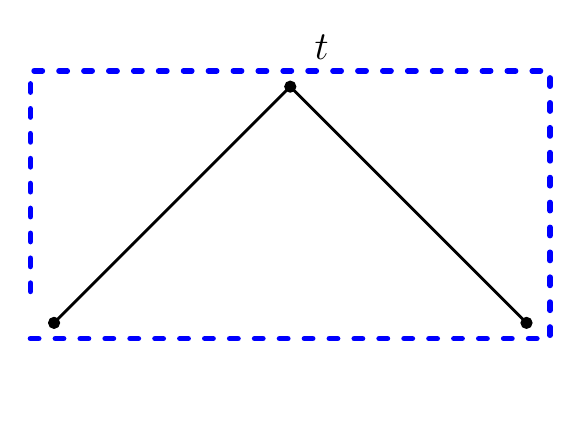
\begin{tikzpicture}[line cap=round,line join=round,>=triangle 45,x=1cm,y=1cm]
%\clip(-7.415949195666677,-4.979207164201812) rectangle (6.110862528225963,7.380468149885891);
\draw [line width=1pt] (3,4)-- (1,2);
\draw [line width=1pt] (3,4)-- (5,2);
%\draw [line width=1pt] (1,2)-- (2,1);
\draw [line width=1pt] (1,2)-- (0,1);
%\draw [line width=1pt] (2,1)-- (1.5,0);
%\draw [line width=1pt] (2,1)-- (2.5,0);
\draw [line width=1pt] (5,2)-- (6,1);
%\draw [line width=1pt] (5,2)-- (4,1);
%\draw [line width=1pt] (0,1)-- (0.5,0);
%\draw [line width=1pt] (0,1)-- (-0.5,0);
\begin{scriptsize}

\tikzstyle{mydashed}= [dash pattern=on 3pt off 6pt];
\draw [line width=2pt, color=blue, mydashed] (-0.3,0.8)--(6.3,0.8)--(6.3,4.2)--(-0.3,4.2)--(-0.3,1.2);
%\draw [fill=black] (3, 3.5) circle (2pt);
%\draw [fill=black] (3, 2.5) circle (2pt);
\draw [fill=black] (0, 1) circle (2pt);%fgg
\draw [fill=white] (0, 0) node {};%fgg
%\draw [fill = black] (-0.5,0) circle (2pt);
%\draw [fill = black] (0.5,0) circle (2pt);
%\draw [fill=black] (2, 1) circle (2pt);
%\draw [fill=black] (1.5, 0) circle (2pt);%fgdg
%\draw [fill=black] (2.5, 0) circle (2pt);%fgdd
%\draw [fill=black] (2, 1) circle (2pt);%fgd 4, 1
%\draw[color=black] (2.3, 1.2) node {\Large $v_3$};
%\draw [fill=black] (1, 2) circle (2pt);%fg 5,2
%\draw[color=black] (0.7, 2.2) node {\Large $v_1$};
%\draw [fill=black] (1, -2) circle (2pt);
%\draw [fill=black] (2, -3) circle (2pt);
%\draw [fill=black] (5, 2) circle (2pt);%fd
%\draw[color=black] (5.3, 2.2) node {\Large $v_2$};
\draw [fill=black] (6, 1) circle (2pt);%fdd
%\draw [fill=black] (4, 1) circle (2pt);%fdg
%\draw [fill=black] (2, -1) circle (2pt);
%\draw [fill=black] (3, -1.5) circle (2pt);
%\draw [fill=black] (3, -0.5) circle (2pt);
%\draw [fill=black] (4, -1) circle (2pt);
%\draw [fill=black] (5, -2) circle (2pt);
\draw [fill=black] (3, 4) circle (2pt);%t 7,0
\draw[color=black] (3.4, 4.5) node {\Large $t$};
\end{scriptsize}
\end{tikzpicture}}
\caption{The EBT $T_{G \backslash \set{e}}$. Nodes of depth 0 to 1 are framed. Graph $G\backslash \set{e}$ belongs to $\mcald_1$.}
\label{subfig:proofth1_c}
\end{subfigure}
\caption{Illustrating the proof of Theorem~\ref{th:completebinary} on a graph of $\mcalg_3$.}
\label{fig:proofth1}
\end{figure}


For any graph $G \in \mcalg$, we note $\cms\left(G\right)$ the maximum over values $\cms\left(G,E_*\right)$ where $\left(G,E_*\right) \in \mcalr$. This value represents the competitive ratio of \mts es on road maps containing graph $G$. Formally, 
\begin{equation}
\cms\left(G\right) = \min\limits_{A ~\mbox{\scriptsize {MS}}} \max\limits_{\left(G,E_*\right) \in \mcalr} c_A\left(G,E_*\right)
\label{eq:cmsg}
\end{equation}
Theorem~\ref{th:equalcompetitive} states that value $\cms\left(G\right)$ is the same for any graph of $\mcald_k$. In other words, graphs in $\mcald_k$ are all similar regarding the competitiveness of \mts es over them. Let $c_k$ denotes the competitive ratio of \mts es over atlas $\mcalr_k$. The proof gives us a recursive formula of ratio $c_k$.

\begin{theorem}
For any graph $G, G' \in \mcald_k$, $c_{\emph{\scriptsize{MS}}}(G) = c_{\emph{\scriptsize{MS}}}(G') = c_k$.
\label{th:equalcompetitive}
\end{theorem}
\begin{proof}
If $k = 0$, then for every graph of $\mcald_0$, $\cms(G) = c_0 = 1$ because any path the traveler takes is open.
We assume the theorem holds for $k-1$. Let $G \in \mcald_k$. Every leaves of $T_G$ are at depth greater than $k$, so the EBT is complete until depth $k$ : $T_G$ have $2^k$ nodes at depth $k$. For a \mts, we define $(p_i)_{i < 2^k}$ by the probability that the traveler travel by the $\ith{i}$ node at depth $k$.

Given a set of $E_*$ of blocked edges, we associate $J(E_*)$ being the set of node at depth $k$ where each \stpath that travel through this node is not blocked. For any node $v$ of depth $k$, we can construct a set of blocked edges such that $\card{J(E_*)} = 1$. Indeed, given a node $v$ of depth $k$, let $e$ be the edge of the sibling of $v$. By blocking $e$,  $U(e)$, $U(U(e))$ ... $U^{k-1}(e)$, we block respectively $1$, $2$, $4$, ... , $2^{k-1}$ nodes. Every edges being the uncle of another, the blocked nodes are disjoint. So finally, only $v$ is not blocked.

For a given set of blocked edges $E_*$, if $v$ is in $J(E_*)$, then by traveling by $v$, the cost will be $1$. If $v$ is not in $J(E_*)$, the traveler have to turned back and choose another path with a road map with $k-1$ blocked edges. Theorem~\ref{th:completebinary} we saw that $G$ without the cut edge is in $\mcald_{k-1}$, so the cost will be at most $2 + c_{k-1}$ by hypothesis. Formally,
\[
c_A(G, E_*) \leq \left(\sum_{j\in J(E_*)} p_j\right)\times 1 + \left(\sum_{j\notin J(E_*)}p_j\right)\times (2+c_{k-1})
\]
We remark that $1 < 2 + c_{k-1}$ so the greater $J(E_*)$ is, the lower $c_A(G, E_*)$ will be. Thus, we remark that for $E_*$ in $\mcalf'$, the inequality above is an equality. So for each $E_*$, it exists $E' \in _mcalf$ such that $c_A(G, E_*) \leq c_A(G, E')$. Finally :
\[
c_A(G, \mcalr_k) = \max_{j < 2^k} p_j + (1-p_j)(2+c_{k-1}) = p_{min} + (1-p_{min})(2+c_{k-1})
\]
with $p_{min}$ the lowest probability. However, $p_{min} \leq \frac{1}{2^k}$ and $c_A(G, \mcalr_k)$ minimum for $p_{min}$ maximum, so $p_{min} = \frac{1}{2^k}$. The result is that $c_{\mts}(G)$ only depend on $k$ and $c_k = \cfrac{1}{2^k} + \left(1-\cfrac{1}{2^k}\right)\left(2+c_{k-1}\right)$
\end{proof}

Theorem~\ref{th:equalcompetitive} give us that for each $k$, the competitive ratio of a \mts can not be lower than $c_k$. The competitiveness of \mts are given by the study of $c$.
To study $c$, first we remark that :
\[
c_k - c_{k-1} = 2 - \cfrac{1}{2^{k}} - \cfrac{c_{k-1}}{2^{k}}
\]
By summing this expression from $j = 1$ to $k$ we obtain :
\[
c_k = 2k+\cfrac{1}{2^k}-\sum_{j=0}^{k-1}\cfrac{c_j}{2^{j+1}}
\]
It came that $c_k \leq 2k+1$ and so the serie is convergent. So finally, $c_k = 2k + O(1)$

%%%%%CONCLUSION%%%%%%%
\section{Conclusion and further work} \label{sec:conclusion}

We studied the competitiveness of the \mts es for the \kctp. In this context, an \mts ~is a strategy which does not make decisions referring to the anterior moves of the traveller, in other words, the nodes the traveller visited until his current position.

%Then, we constructed a series of \kctp{} instances, called road atlases and noted $\mcals_k$. Identifying an efficient randomized \mts{}es becomes harder when $k$ tends to infinity. We foremost concluded that a randomized  \mts{}~cannot reach a competitive ratio smaller than $\frac{10}{9}k+1 = 3.22(2)$ on road atlas $\mcals_2$. We extended our reasoning to larger atlases and established that the competitive ratio of randomized \mts es on maps with $k$ blockages is larger than $\left(3-\sqrt{3}\right)k + 1 \approx 1.268k+1$. That is to say that we identified an upper bound on the competitive ratio of randomized \mts{}es which is significantly higher than the existing one $k+1$. Now, if the objective is to find a strategy with a competitive ratio smaller than $k\beta + 1$, one shall study strategies which are not memoryless.

%The main issue that, in our opinion, needs further investigation, is the improvement of the new lower bound. There are, potentially, two ways to do this. The first one is the modification of road atlases $\mcals_k$ to make \mts es be less efficient on them. The second possibility consists in increasing the lower bound of the competitive ratio by introducing new properties of \mts es, more advantageous for bounding, on the road atlas $\mcals_k$. Other possible future work could be to design a randomized strategy with ratio less than $1.268k+1$ and which is not memoryless, or to design a family of maps such that there exists a randomized strategy which, applied on it, has a ratio $k+1$.
%Then, the difference of competitiveness between \mts es and other strategies is still open: is there a randomized strategy, which is not \mts , such that its competitive ratio is inferior to $\left(3 - \sqrt{3}\right)k+1$ ? We also wonder if there exists a randomized \mts ~whose competitive ratio is inferior to $2k+1$, which is the optimal competitive ratio of deterministic strategies.
% Another track is to study the competitiveness of randomized strategies (and particularly \mts es) on specific graphs, as Bender {\em et al.\/} did it with graphs composed of node-disjoint paths.

\bibliographystyle{plain}
\bibliography{mctp.bib}



\end{document}
